\documentclass[aspectratio=169,12pt]{beamer}
\usepackage{eafitml}
\usepackage{colortbl}

% ---------------------------------------------------------------- local macros
\setbeamertemplate{section in toc}{\leavevmode{\color{mlgold}\inserttocsectionnumber.}~\inserttocsection\par}
\setbeamertemplate{subsection in toc}{\leavevmode\leftskip=2.2em\small\mdseries\inserttocsubsection\par}
\setbeamerfont{section in toc}{series=\bfseries,size=\normalsize}

\newtcolorbox{goldbox}[1][]{enhanced,sharp corners,boxrule=0pt,frame hidden,
  colback=mltealbg,colbacktitle=mlgold,coltitle=white,
  fonttitle=\bfseries\small,left=4pt,right=4pt,top=2pt,bottom=2pt,
  toptitle=1pt,bottomtitle=1pt,before skip=4pt,after skip=4pt,title={#1}}

% keep beamer's compact list spacing inside \small / \footnotesize
\makeatletter
\let\ml@beamerlisti\@listi
\expandafter\apptocmd\csname small \endcsname{\let\@listi\ml@beamerlisti}{}{}
\expandafter\apptocmd\csname footnotesize \endcsname{\let\@listi\ml@beamerlisti}{}{}
\makeatother
\newcolumntype{L}[1]{>{\raggedright\arraybackslash}p{#1}}
\newcommand{\colhead}[1]{\textbf{#1}\par\vspace{2pt}}
\newcommand{\hrow}{\rowcolor{mlcream}}
\renewcommand{\arraystretch}{1.15}
\newcommand{\fig}[2][width=\linewidth]{\includegraphics[#1]{figures/#2}}
\usetikzlibrary{decorations.pathreplacing,matrix,arrows.meta,positioning}
\lstset{numbers=left,numberstyle=\tiny\color{mlgray},numbersep=8pt,backgroundcolor={}}

\title[Reducción de dimensionalidad]{Reducción de dimensionalidad}
\subtitle{Aprendizaje Automático · Sesión 5}
\author[Aprendizaje Automático]{Andrés Vásquez Restrepo\\[2pt]{\normalfont\small\texttt{avasquezr3@eafit.edu.co}}}
\institute{SI7009 - 1 (5553)\\Universidad EAFIT}
\date{2026-2 -- Medellín}
\titlegraphic{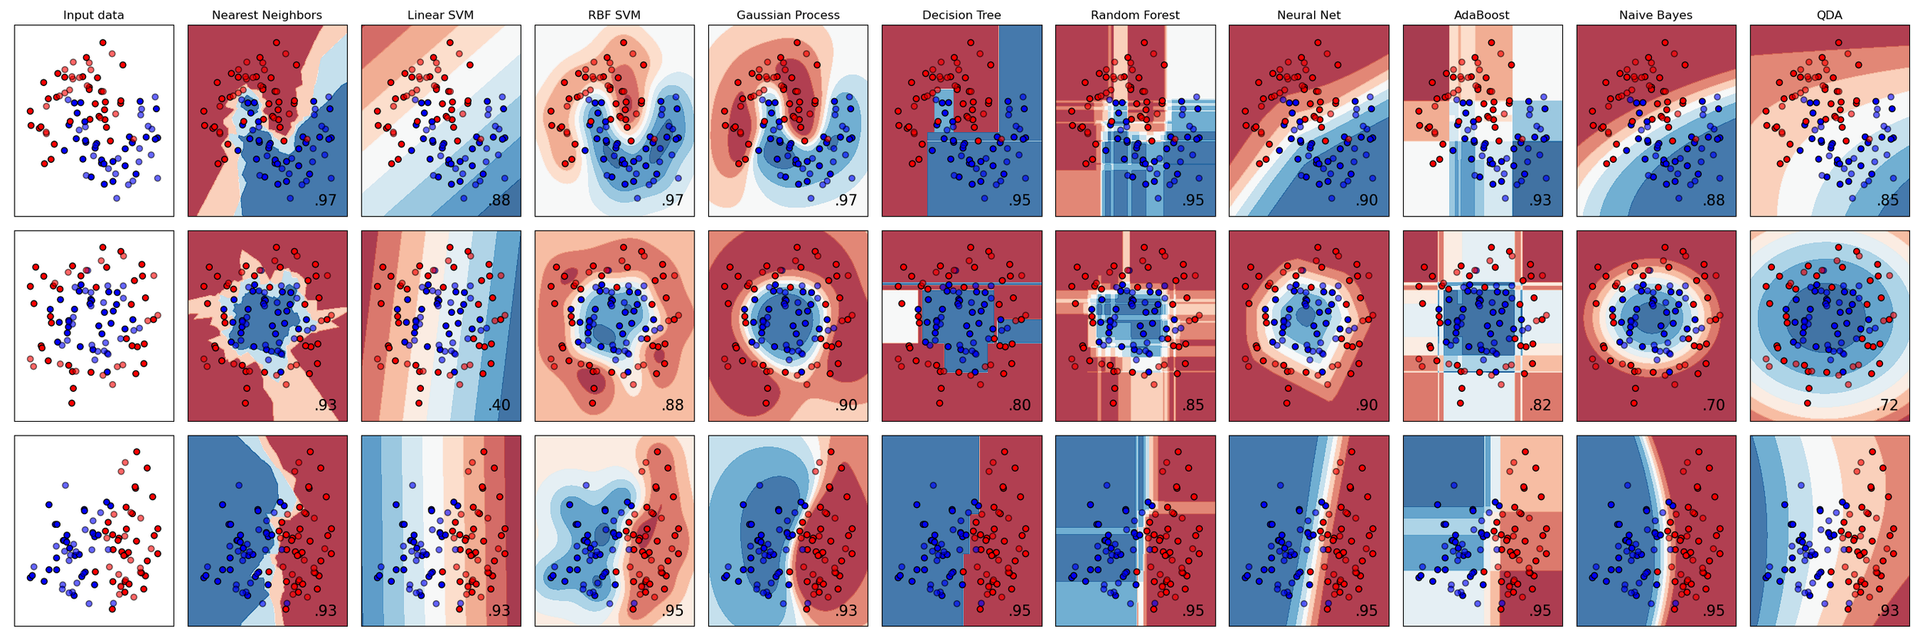
\includegraphics[width=5cm]{figures/img_p001_01.png}}

\begin{document}

% ============================================================ A1-A3 apertura
\titleframe
\addtocounter{framenumber}{1}

\begin{frame}{Contenido}
  \tableofcontents
\end{frame}

\begin{frame}{Dónde quedamos}
  \begin{columns}[T]
    \begin{column}{0.5\textwidth}
      \colhead{Sesiones 1 a 4}
      \small
      \begin{itemize}
        \item siempre hubo un target $y$: fraude, demanda, preferencia;
        \item el modelo se juzgaba contra ese $y$ (PR-AUC, MASE, NDCG).
      \end{itemize}
      \vspace{4pt}
      \colhead{Hoy y mañana}
      \begin{itemize}
        \item no hay $y$: la pregunta es \textbf{qué estructura tiene $X$};
        \item no hay una métrica obvia contra la cual comparar.
      \end{itemize}
    \end{column}
    \begin{column}{0.44\textwidth}
      \begin{keybox}[Unidad 3]
        \small Tabla $\rightarrow$ \textbf{representación} (S5) $\rightarrow$ grupos, anomalías y drift (S6).
      \end{keybox}
      \begin{notebox}[Caso de las dos sesiones]
        \small Vendedores de \textbf{Olist}, construidos con SQL sobre la misma base DuckDB del taller. El taller pide clientes: mismo método, otra unidad.
      \end{notebox}
    \end{column}
  \end{columns}
\end{frame}

% ============================================================ 1. por qué reducir
\section{Por qué reducir dimensión}
\sectionframe{Por qué reducir dimensión}

\begin{frame}{Una fila es un punto}
  \centering\scriptsize
  \setlength{\tabcolsep}{3.5pt}
  \begin{tabular}{@{}l r r r r r r r r@{}}
    \toprule
    \hrow & \textbf{ventas} & \textbf{órdenes} & \textbf{ticket} & \textbf{flete/precio} & \textbf{categ.} & \textbf{retraso} & \textbf{días transp.} & \textbf{calif.} \\
    \midrule
    A & 293 & 6 & 49 & 34\,\% & 2 & 0\,\% & 1,1 & 4,67 \\
    B & 1.774 & 9 & 197 & 8\,\% & 1 & 0\,\% & 0,8 & 4,89 \\
    C & 165.563 & 317 & 522 & 4\,\% & 7 & 5\,\% & 1,3 & 4,37 \\
    \bottomrule
  \end{tabular}
  \raggedright\small
  \vspace{6pt}
  \begin{columns}[T]
    \begin{column}{0.48\textwidth}
      Cada vendedor es un vector $x \in \mathbb{R}^8$. Parecido = cerca:
      \[ d(x,x') = \lVert x - x' \rVert_2 = \sqrt{\textstyle\sum_j (x_j - x'_j)^2} \]
    \end{column}
    \begin{column}{0.48\textwidth}
      \begin{rulebox}[Sin preparar los datos]
        \small $d(A,B) \approx 1.481$ y $d(A,C) \approx 165.270$: la distancia es casi solo \textbf{ventas}. Las otras 7 columnas no cuentan.
      \end{rulebox}
    \end{column}
  \end{columns}
  \vspace{2pt}
  \footnotesize\color{mlgray} 1.740 vendedores con $\geq 3$ órdenes entregadas antes de 2018-06-01.
\end{frame}

\begin{frame}{La maldición de la dimensionalidad}
  \begin{columns}[c]
    \begin{column}{0.58\textwidth}
      \fig{r2_distance_concentration.png}
    \end{column}
    \begin{column}{0.4\textwidth}
      \footnotesize
      Desde un punto, compare el vecino \textbf{más cercano} con el \textbf{más lejano}:
      \[ \frac{d_{\max}-d_{\min}}{d_{\min}} \]
      \begin{itemize}
        \item $p=2$: el lejano está 130 veces más lejos;
        \item $p=100$: solo un 32\,\% más lejos;
        \item $p=1000$: un 11\,\%.
      \end{itemize}
      \begin{keybox}
        \footnotesize Con muchas dimensiones todos quedan casi a la misma distancia: ``vecino'' pierde sentido.
      \end{keybox}
    \end{column}
  \end{columns}
\end{frame}

\begin{frame}{Cuatro usos de la reducción}
  \centering\footnotesize
  \begin{tabular}{@{}L{0.2\textwidth} L{0.24\textwidth} L{0.44\textwidth}@{}}
    \toprule
    \hrow \textbf{Uso} & \textbf{Método típico} & \textbf{Cómo se evalúa} \\
    \midrule
    Visualizar & t-SNE, UMAP, PCA 2D & ¿Se conservan los vecinos? ¿Es estable? \\
    Comprimir & PCA & Varianza explicada, error de reconstrucción \\
    Quitar ruido y colinealidad & PCA & Desempeño del modelo siguiente \\
    Preprocesar para clustering o modelos & PCA, UMAP a 5--10 dims & Métrica de la tarea siguiente, con CV \\
    \bottomrule
  \end{tabular}
  \raggedright
  \begin{keybox}
    \small No hay ``mejor reducción'' en abstracto: hay mejor reducción \textbf{para un uso}.
  \end{keybox}
\end{frame}

\begin{frame}{Selección frente a extracción}
  \begin{columns}[T]
    \begin{column}{0.48\textwidth}
      \begin{defbox}[Seleccionar variables]
        \small Quedarse con un subconjunto de las columnas originales.
        \begin{itemize}
          \item[+] interpretables: ``ventas'' sigue siendo ventas;
          \item[--] pierde la información que solo existe en combinaciones;
          \item[--] dos columnas redundantes siguen ahí.
        \end{itemize}
      \end{defbox}
    \end{column}
    \begin{column}{0.48\textwidth}
      \begin{defbox}[Extraer variables nuevas]
        \small Construir $z = f(x)$ con menos dimensiones.
        \begin{itemize}
          \item[+] compacta la información de muchas columnas;
          \item[+] elimina redundancia;
          \item[--] cada $z_j$ hay que interpretarla (PCA) o no se puede (t-SNE).
        \end{itemize}
      \end{defbox}
    \end{column}
  \end{columns}
  \vspace{4pt}
  \small Hoy: \textbf{extracción}. Lineal (PCA) y no lineal (t-SNE, UMAP).
\end{frame}

\begin{frame}{El escalado decide la geometría}
  \begin{columns}[c]
    \begin{column}{0.62\textwidth}
      \fig{r5_scaling.png}
    \end{column}
    \begin{column}{0.36\textwidth}
      \footnotesize
      \begin{itemize}
        \item ventas va de 30 a 500.000 BRL: domina cualquier distancia;
        \item \texttt{log1p} para variables sesgadas (ventas, órdenes, ticket, categorías, días);
        \item luego \texttt{StandardScaler}: media 0, desviación 1.
      \end{itemize}
      \begin{rulebox}
        \footnotesize En no supervisado el preprocesamiento \textbf{es} parte del modelo: otra transformación, otros vecinos.
      \end{rulebox}
    \end{column}
  \end{columns}
\end{frame}

% ============================================================ 2. PCA
\section{PCA}
\sectionframe{PCA: proyección lineal}

\begin{frame}{La idea}
  \begin{columns}[c]
    \begin{column}{0.42\textwidth}
      \centering\fig[width=\linewidth,keepaspectratio,height=0.7\textheight]{p1_pca_idea.png}
    \end{column}
    \begin{column}{0.54\textwidth}
      \small
      \begin{enumerate}
        \item centrar los datos;
        \item buscar la dirección donde la nube \textbf{se estira más} (PC1);
        \item la siguiente dirección, perpendicular a la anterior, que más se estira (PC2), y así;
        \item proyectar cada punto sobre las primeras $k$ direcciones.
      \end{enumerate}
      \begin{keybox}
        \small PCA es una \textbf{rotación} de ejes seguida de quedarse con los primeros $k$. Nada más.
      \end{keybox}
    \end{column}
  \end{columns}
\end{frame}

\begin{frame}{El problema de optimización}
  \small Con $X$ centrada y $\Sigma = \frac{1}{n-1}X^\top X$, la varianza de la proyección $z = X\mathbf{w}$ es $\mathbf{w}^\top \Sigma \mathbf{w}$:
  \[ \mathbf{w}_1 = \arg\max_{\lVert \mathbf{w} \rVert = 1} \ \mathbf{w}^\top \Sigma\, \mathbf{w} \]
  Con un multiplicador de Lagrange, $\mathcal{L} = \mathbf{w}^\top\Sigma\mathbf{w} - \lambda(\mathbf{w}^\top\mathbf{w}-1)$, y derivando:
  \[ \Sigma\, \mathbf{w} = \lambda\, \mathbf{w} \qquad\Rightarrow\qquad \operatorname{Var}(X\mathbf{w}) = \mathbf{w}^\top\Sigma\mathbf{w} = \lambda \]
  \begin{columns}[T]
    \begin{column}{0.48\textwidth}
      \begin{defbox}[Componentes]
        \small Los \textbf{eigenvectores} de $\Sigma$, ordenados por eigenvalor.
      \end{defbox}
    \end{column}
    \begin{column}{0.48\textwidth}
      \begin{defbox}[Varianza de cada componente]
        \small El \textbf{eigenvalor} $\lambda_j$. Suman la varianza total.
      \end{defbox}
    \end{column}
  \end{columns}
\end{frame}

\begin{frame}{PCA a mano: el mini-mundo}
  \begin{columns}[c]
    \begin{column}{0.4\textwidth}
      \centering
      \begin{tikzpicture}[scale=0.48]
        \draw[step=1,mlgray!25,very thin] (0,0) grid (9,8);
        \draw[-{Stealth},mlgray] (0,0) -- (9.3,0); \draw[-{Stealth},mlgray] (0,0) -- (0,8.3);
        \draw[eafitblue,very thick,dashed] (4.33-5*0.79,4-5*0.61) -- (4.33+5*0.79,4+5*0.61) node[right,font=\scriptsize]{PC1};
        \foreach \n/\x/\y in {A/1/2,B/2/1,C/2/3,D/6/5,E/7/7,F/8/6}{
          \fill[mlteal] (\x,\y) circle (4pt); \node[font=\scriptsize,above left] at (\x,\y) {\n};}
        \fill[mlred] (4.33,4) circle (3pt) node[below right,font=\scriptsize]{$\bar x$};
      \end{tikzpicture}
    \end{column}
    \begin{column}{0.58\textwidth}
      \small
      \begin{enumerate}
        \item media: $\bar x = (4{,}33;\ 4{,}00)$
        \item covarianza: $\Sigma = \begin{pmatrix} 9{,}07 & 6{,}60 \\ 6{,}60 & 5{,}60\end{pmatrix}$
        \item eigenvalores: $\lambda_1 = 14{,}16$, $\lambda_2 = 0{,}51$
        \item PC1: $\mathbf{w}_1 \approx (0{,}79;\ 0{,}61)$
        \item PC1 explica $\frac{14{,}16}{14{,}67} = $ \textbf{96,5\,\%}
      \end{enumerate}
      \footnotesize
      \begin{tabular}{@{}l c c c c c c@{}}
        \toprule
        \hrow & A & B & C & D & E & F \\
        \midrule
        $z_1$ & $-3{,}86$ & $-3{,}68$ & $-2{,}46$ & $1{,}93$ & $3{,}94$ & $4{,}12$ \\
        \bottomrule
      \end{tabular}
    \end{column}
  \end{columns}
  \vspace{2pt}
  \small Un solo número por punto conserva casi todo: separa {A, B, C} de {D, E, F}. (Mañana volvemos a estos 6 puntos.)
\end{frame}

\begin{frame}{PCA vía SVD}
  \centering
  \begin{tikzpicture}[mat/.style={draw=mlteal,fill=mltealbg,minimum height=1.6cm,align=center,font=\small}]
    \node[mat,minimum width=1.4cm] (X) {$X_c$\\{\scriptsize $n\times p$}};
    \node[right=0.2cm of X] (eq) {$=$};
    \node[mat,minimum width=1.4cm,right=0.2cm of eq] (U) {$U$\\{\scriptsize $n\times p$}};
    \node[mat,minimum width=1.0cm,minimum height=1.0cm,right=0.2cm of U] (S) {$S$\\{\scriptsize diag.}};
    \node[mat,minimum width=1.4cm,minimum height=1.0cm,right=0.2cm of S] (V) {$V^\top$\\{\scriptsize $p\times p$}};
  \end{tikzpicture}
  \vspace{6pt}
  \raggedright\small
  \begin{itemize}
    \item componentes principales = filas de $V^\top$ (columnas de $V$);
    \item varianzas: $\lambda_j = s_j^2 / (n-1)$;
    \item coordenadas: $Z = X_c V_k = U_k S_k$.
  \end{itemize}
  \begin{goldbox}[Por qué las librerías usan SVD y no $\Sigma$]
    \small No forma $X^\top X$ (pierde precisión numérica). Con $n$ o $p$ grandes, \texttt{svd\_solver='randomized'} calcula solo los primeros $k$ componentes.
  \end{goldbox}
\end{frame}

\begin{frame}{Varianza explicada y scree plot}
  \begin{columns}[c]
    \begin{column}{0.6\textwidth}
      \fig{p5_scree.png}
    \end{column}
    \begin{column}{0.38\textwidth}
      \small
      \[ \text{EVR}_j = \frac{\lambda_j}{\sum_l \lambda_l} \]
      \begin{itemize}
        \item PC1: 30\,\%, PC2: 23\,\%, PC3: 20\,\%;
        \item 4 componentes $\rightarrow$ 82\,\%;
        \item PC8 $\approx 0$: $\log(\text{ventas}) \approx \log(\text{órdenes}) + \log(\text{ticket})$. Redundancia exacta.
      \end{itemize}
      \begin{keybox}
        \small Criterios: 80--90\,\% acumulado, el codo, o el $k$ que mejor sirve a la tarea siguiente.
      \end{keybox}
    \end{column}
  \end{columns}
\end{frame}

\begin{frame}{Leer los loadings}
  \begin{columns}[c]
    \begin{column}{0.52\textwidth}
      \centering\fig[width=\linewidth,keepaspectratio,height=0.74\textheight]{p6_loadings.png}
    \end{column}
    \begin{column}{0.46\textwidth}
      \footnotesize
      \begin{goldbox}[PC1 (30\,\%): tamaño del vendedor]
        \footnotesize $+$ ventas, órdenes, ticket, categorías; $-$ flete relativo.
      \end{goldbox}
      \begin{goldbox}[PC2 (23\,\%): mala experiencia de entrega]
        \footnotesize $+$ \% retraso, días a la transportadora; $-$ calificación.
      \end{goldbox}
      \begin{rulebox}[Cuidado]
        \footnotesize El signo es arbitrario. Nombrar un componente es una \textbf{hipótesis} que hay que defender con los datos.
      \end{rulebox}
    \end{column}
  \end{columns}
\end{frame}

\begin{frame}{Reconstrucción}
  \begin{columns}[c]
    \begin{column}{0.55\textwidth}
      \fig{p7_reconstruction.png}
    \end{column}
    \begin{column}{0.43\textwidth}
      \footnotesize
      Volver al espacio original con $k$ componentes:
      \[ \hat{x} = \bar{x} + V_k V_k^\top (x - \bar{x}) \]
      \begin{itemize}
        \item el error baja con $k$ y es 0 con $k=p$;
        \item con $k=4$: MSE = 0,18 (sobre datos estandarizados).
      \end{itemize}
      \begin{keybox}[Puente a la S6]
        \footnotesize Quien \textbf{se reconstruye mal} no se parece al resto: el error sirve como score de anomalía.
      \end{keybox}
    \end{column}
  \end{columns}
\end{frame}

\begin{frame}{PCA dentro del pipeline}
  \centering
  \begin{tikzpicture}[node distance=0.35cm,
      st/.style={fill=mlcream,minimum height=0.9cm,align=center,font=\footnotesize,text width=2.1cm},
      arr/.style={-{Stealth[length=2mm]},thick,eafitblue}]
    \node[st] (a) {log + escalado};
    \node[st,right=of a,fill=eafitsky] (b) {PCA\\$k$ componentes};
    \node[st,right=of b] (c) {modelo o clustering};
    \node[st,right=of c] (d) {métrica en validación};
    \draw[arr] (a) -- (b); \draw[arr] (b) -- (c); \draw[arr] (c) -- (d);
    \draw[decorate,decoration={brace,amplitude=5pt,mirror},mlgray] (a.south west) -- (c.south east)
      node[midway,below=6pt,font=\scriptsize,text=mlgray] {\texttt{Pipeline}: \texttt{fit} solo con train};
  \end{tikzpicture}
  \vspace{4pt}
  \raggedright\small
  \begin{columns}[T]
    \begin{column}{0.48\textwidth}
      \begin{rulebox}[Leakage, otra vez (S1)]
        \small Ajustar PCA o el escalador con todos los datos usa información del test para construir las features.
      \end{rulebox}
    \end{column}
    \begin{column}{0.48\textwidth}
      \begin{keybox}[Hiperparámetro]
        \small $k$ se elige con CV como cualquier otro hiperparámetro (S2): \texttt{pca\_\_n\_components} dentro de la búsqueda.
      \end{keybox}
    \end{column}
  \end{columns}
\end{frame}

\begin{frame}{Cuándo PCA falla}
  \fig{p9_pca_failures.png}
  \small
  \begin{columns}[T]
    \begin{column}{0.32\textwidth}\centering\textbf{No lineal}\\{\footnotesize ninguna recta separa los anillos}\end{column}
    \begin{column}{0.32\textwidth}\centering\textbf{Outliers}\\{\footnotesize 3 puntos giran PC1 casi 90°}\end{column}
    \begin{column}{0.32\textwidth}\centering\textbf{Varianza $\neq$ relevancia}\\{\footnotesize lo que separa las clases está en PC2}\end{column}
  \end{columns}
\end{frame}

\begin{frame}[fragile]{PCA en código}
  \begin{columns}[T]
    \begin{column}{0.56\textwidth}
\begin{lstlisting}
from sklearn.pipeline import make_pipeline
from sklearn.preprocessing import (
    FunctionTransformer, StandardScaler)
from sklearn.decomposition import PCA

pca_pipe = make_pipeline(
    FunctionTransformer(np.log1p),
    StandardScaler(),
    PCA(n_components=0.9),  # 90 % var.
)
Z = pca_pipe.fit_transform(X_sellers)

pca = pca_pipe[-1]
pca.explained_variance_ratio_
pca.components_          # loadings
pca.inverse_transform(Z) # reconstruccion
\end{lstlisting}
    \end{column}
    \begin{column}{0.4\textwidth}
      \small
      \begin{itemize}
        \item \texttt{n\_components} entero = $k$; fracción = varianza mínima;
        \item \texttt{components\_} tiene forma $(k, p)$: una fila por componente;
        \item aplique \texttt{log1p} solo a las columnas sesgadas (\texttt{ColumnTransformer}).
      \end{itemize}
    \end{column}
  \end{columns}
\end{frame}

% ============================================================ 3. más allá de lo lineal
\section{Más allá de lo lineal}
\sectionframe{Más allá de lo lineal}

\begin{frame}{La hipótesis de la variedad}
  \centering\fig[width=\linewidth,keepaspectratio,height=0.5\textheight]{m1_swissroll.png}
  \raggedright\small
  \begin{itemize}
    \item los datos de alta dimensión suelen vivir cerca de una \textbf{superficie} de pocas dimensiones;
    \item en el swiss roll, dos puntos cercanos en línea recta pueden estar lejos \textbf{sobre la superficie};
    \item PCA solo rota y proyecta: deja la espiral enrollada.
  \end{itemize}
\end{frame}

\begin{frame}{Global frente a local}
  \centering\small
  \begin{tabular}{@{}l L{0.32\textwidth} L{0.38\textwidth}@{}}
    \toprule
    \hrow \textbf{Método} & \textbf{Qué preserva} & \textbf{Qué distorsiona} \\
    \midrule
    PCA & varianza global, distancias grandes & estructura no lineal, vecindarios finos \\
    Kernel PCA, Isomap & estructura no lineal global & costo $O(n^2)$ o más; sensibles a parámetros \\
    t-SNE & vecindarios locales & distancias entre grupos, tamaños, densidades \\
    UMAP & vecindarios locales y algo de lo global & distancias globales (menos que t-SNE) \\
    \bottomrule
  \end{tabular}
  \raggedright
  \begin{keybox}
    \small En 2D no cabe todo. Cada método \textbf{elige qué sacrificar}. Antes de leer una figura hay que saber qué sacrificó.
  \end{keybox}
\end{frame}

% ============================================================ 4. t-SNE
\section{t-SNE}
\sectionframe{t-SNE}

\begin{frame}{Vecindades como probabilidades}
  \begin{columns}[c]
    \begin{column}{0.36\textwidth}
      \centering
      \begin{tikzpicture}[scale=0.9]
        \fill[eafitsky!60] (0,0) circle (1.4);
        \fill[eafitsky] (0,0) circle (0.75);
        \foreach \x/\y in {0.4/0.3,-0.5/0.2,0.2/-0.6,-0.3/-0.4}{\fill[mlteal] (\x,\y) circle (2.5pt);}
        \foreach \x/\y in {1.1/0.6,-1.0/0.9,0.9/-1.0}{\fill[mlteal!60] (\x,\y) circle (2.5pt);}
        \foreach \x/\y in {2.0/0.3,-1.9/-1.1,1.6/1.6}{\fill[mlgray!60] (\x,\y) circle (2.5pt);}
        \fill[mlred] (0,0) circle (3pt) node[below=2pt,font=\scriptsize]{$x_i$};
      \end{tikzpicture}
      \\[2pt]{\scriptsize vecinos cercanos: $p_{j|i}$ alta}
    \end{column}
    \begin{column}{0.62\textwidth}
      \small En el espacio original, la probabilidad de que $x_i$ ``elija'' a $x_j$ como vecino:
      \[ p_{j|i} = \frac{\exp\!\left(-\lVert x_i - x_j\rVert^2 / 2\sigma_i^2\right)}{\sum_{k\neq i}\exp\!\left(-\lVert x_i - x_k\rVert^2 / 2\sigma_i^2\right)} \]
      Simetrizada:
      \[ p_{ij} = \frac{p_{j|i} + p_{i|j}}{2n} \]
      \begin{keybox}
        \small t-SNE convierte distancias en una distribución de ``quién es vecino de quién''.
      \end{keybox}
    \end{column}
  \end{columns}
\end{frame}

\begin{frame}{Perplexity}
  \small Cada punto tiene su propio ancho $\sigma_i$. Se ajusta para que la entropía de $P_i$ dé una perplexity fija:
  \[ \text{Perp}(P_i) = 2^{H(P_i)}, \qquad H(P_i) = -\sum_j p_{j|i}\log_2 p_{j|i} \]
  \begin{columns}[T]
    \begin{column}{0.48\textwidth}
      \begin{defbox}[Lectura]
        \small Perplexity $\approx$ \textbf{número efectivo de vecinos} que mira cada punto. Valores típicos: 5 a 50.
      \end{defbox}
    \end{column}
    \begin{column}{0.48\textwidth}
      \begin{defbox}[Densidad adaptativa]
        \small En zonas densas $\sigma_i$ es pequeño; en zonas ralas, grande. Por eso t-SNE \textbf{borra} las diferencias de densidad.
      \end{defbox}
    \end{column}
  \end{columns}
\end{frame}

\begin{frame}{Student-t y el problema de aglomeración}
  \begin{columns}[c]
    \begin{column}{0.56\textwidth}
      \fig{t3_gauss_vs_t.png}
    \end{column}
    \begin{column}{0.42\textwidth}
      \small En 2D no caben todos los vecinos de un punto de alta dimensión: si se usa otra gaussiana, todo se amontona en el centro.
      \vspace{4pt}

      En el embedding $y$:
      \[ q_{ij} = \frac{(1+\lVert y_i - y_j\rVert^2)^{-1}}{\sum_{k\neq l}(1+\lVert y_k - y_l\rVert^2)^{-1}} \]
      \begin{keybox}
        \small La cola pesada deja que puntos moderadamente lejanos se separen mucho. Por eso aparecen ``islas''.
      \end{keybox}
    \end{column}
  \end{columns}
\end{frame}

\begin{frame}{El objetivo: divergencia KL}
  \[ C = \text{KL}(P \,\Vert\, Q) = \sum_{i\neq j} p_{ij}\,\log\frac{p_{ij}}{q_{ij}} \]
  \begin{columns}[T]
    \begin{column}{0.48\textwidth}
      \begin{goldbox}[Asimétrica]
        \small $p_{ij}$ alto y $q_{ij}$ bajo (separar vecinos): \textbf{costo alto}.\\
        $p_{ij}$ bajo y $q_{ij}$ alto (juntar lejanos): \textbf{casi gratis}.
      \end{goldbox}
    \end{column}
    \begin{column}{0.48\textwidth}
      \begin{goldbox}[Optimización]
        \small Descenso de gradiente sobre las $y_i$; \emph{early exaggeration} al inicio; inicializar con PCA da resultados más estables.
      \end{goldbox}
    \end{column}
  \end{columns}
  \begin{keybox}
    \small t-SNE se esfuerza por mantener juntos a los vecinos. No le importa dónde quedan los grupos entre sí.
  \end{keybox}
\end{frame}

\begin{frame}{Mismos datos, distinta perplexity}
  \fig{t5_perplexity.png}
  \small 1.740 vendedores, mismas 8 variables, color = $\log_{10}$(ventas). Cambia el tamaño de las ``islas'', su forma y la distancia entre ellas.
  \begin{rulebox}
    \small Si una conclusión cambia con la perplexity, no era una conclusión sobre los datos.
  \end{rulebox}
\end{frame}

\begin{frame}{Lecturas permitidas y prohibidas}
  \begin{columns}[T]
    \begin{column}{0.48\textwidth}
      \colhead{Se puede leer}
      \small
      \begin{itemize}
        \item quién es vecino de quién;
        \item gradientes de una variable a lo largo del mapa;
        \item puntos aislados para inspeccionar.
      \end{itemize}
    \end{column}
    \begin{column}{0.48\textwidth}
      \colhead{No se puede leer}
      \small
      \begin{itemize}
        \item distancia entre grupos;
        \item tamaño o densidad de un grupo;
        \item número de grupos;
        \item ejes (no significan nada).
      \end{itemize}
    \end{column}
  \end{columns}
  \vspace{4pt}
  \begin{rulebox}[Limitaciones prácticas]
    \small No tiene \texttt{transform}: un punto nuevo obliga a recalcular todo. Costo $O(n \log n)$ con Barnes--Hut. Pensado para visualizar en 2D o 3D, no para crear features.
  \end{rulebox}
\end{frame}

% ============================================================ 5. UMAP
\section{UMAP}
\sectionframe{UMAP}

\begin{frame}{Un grafo de vecinos difuso}
  \begin{columns}[c]
    \begin{column}{0.38\textwidth}
      \centering
      \begin{tikzpicture}[scale=0.9,v/.style={circle,fill=mlteal,inner sep=2pt}]
        \node[v,fill=mlred] (i) at (0,0) {};
        \node[v] (a) at (0.8,0.5) {}; \node[v] (b) at (-0.7,0.7) {}; \node[v] (c) at (0.3,-0.9) {};
        \node[v] (d) at (1.9,1.2) {}; \node[v] (e) at (-1.8,-0.6) {}; \node[v] (f) at (1.6,-0.6) {};
        \draw[eafitblue,line width=2.4pt] (i) -- (a);
        \draw[eafitblue,line width=1.6pt] (i) -- (b);
        \draw[eafitblue,line width=1.0pt] (i) -- (c);
        \draw[eafitblue!50,line width=0.8pt] (a) -- (d); \draw[eafitblue!50,line width=0.8pt] (c) -- (f);
        \draw[eafitblue!50,line width=0.8pt] (b) -- (e);
        \node[below=3pt,font=\scriptsize] at (i) {$x_i$};
      \end{tikzpicture}
      \\{\scriptsize grosor = peso $w_{ij}$}
    \end{column}
    \begin{column}{0.6\textwidth}
      \small
      \begin{enumerate}
        \item buscar los $k$ vecinos más cercanos de cada punto;
        \item pesar cada arista:
          \[ w_{ij} = \exp\!\left(-\frac{d(x_i,x_j) - \rho_i}{\sigma_i}\right) \]
          $\rho_i$ = distancia al vecino más cercano (el más cercano siempre pesa 1);
        \item simetrizar: $w = w_{ij} + w_{ji} - w_{ij}w_{ji}$.
      \end{enumerate}
      \begin{keybox}
        \small Igual que t-SNE, cada punto mide distancias con su propia escala local.
      \end{keybox}
    \end{column}
  \end{columns}
\end{frame}

\begin{frame}{Optimizar el layout}
  \small Buscar posiciones $y_i$ en 2D cuyo grafo se parezca al original, minimizando una cross-entropy:
  \[ C = \sum_{(i,j)} \underbrace{w_{ij}\log\frac{w_{ij}}{v_{ij}}}_{\text{atracción}} + \underbrace{(1-w_{ij})\log\frac{1-w_{ij}}{1-v_{ij}}}_{\text{repulsión}}, \qquad v_{ij} = \left(1 + a\lVert y_i - y_j\rVert^{2b}\right)^{-1} \]
  \begin{columns}[T]
    \begin{column}{0.48\textwidth}
      \begin{goldbox}[Atracción]
        \small Sobre las aristas del grafo: vecinos se acercan.
      \end{goldbox}
    \end{column}
    \begin{column}{0.48\textwidth}
      \begin{goldbox}[Repulsión]
        \small Sobre pares al azar (\emph{negative sampling}): no vecinos se alejan. Esto la hace rápida.
      \end{goldbox}
    \end{column}
  \end{columns}
  \small A diferencia de KL, el segundo término también castiga juntar lo que estaba lejos: UMAP conserva algo más de estructura global.
\end{frame}

\begin{frame}{\texttt{n\_neighbors} y \texttt{min\_dist}}
  \begin{columns}[c]
    \begin{column}{0.64\textwidth}
      \fig{u3_umap_grid.png}
    \end{column}
    \begin{column}{0.34\textwidth}
      \small
      \begin{defbox}[\texttt{n\_neighbors}]
        \small Pocos: estructura muy local, el mapa se rompe en hilos. Muchos: más global, más suave.
      \end{defbox}
      \begin{defbox}[\texttt{min\_dist}]
        \small Qué tan apretados pueden quedar los puntos. 0 = grumos densos (útil para clustering).
      \end{defbox}
      \footnotesize\color{mlgray} Color = $\log_{10}$(ventas).
    \end{column}
  \end{columns}
\end{frame}

\begin{frame}{UMAP frente a t-SNE}
  \centering\small
  \begin{tabular}{@{}L{0.34\textwidth} L{0.26\textwidth} L{0.26\textwidth}@{}}
    \toprule
    \hrow & \textbf{t-SNE} & \textbf{UMAP} \\
    \midrule
    Estructura global & poca & algo más \\
    Datos nuevos & recalcular todo & \texttt{transform()} \\
    Dimensiones de salida & 2 o 3 & cualquiera (p. ej. 10) \\
    Métricas de distancia & euclídea (en la práctica) & cualquiera (coseno, Jaccard\ldots) \\
    Velocidad con $n$ grande & lenta & rápida \\
    Determinista & no & no \\
    \bottomrule
  \end{tabular}
  \raggedright
  \begin{keybox}
    \small Para visualizar, los dos sirven. Para usar el embedding como entrada de otra cosa, UMAP.
  \end{keybox}
\end{frame}

\begin{frame}{UMAP antes de clustering}
  \begin{columns}[T]
    \begin{column}{0.48\textwidth}
      \colhead{Práctica común}
      \small
      \begin{itemize}
        \item UMAP a 5--10 dimensiones (no 2);
        \item \texttt{min\_dist=0} para grumos densos;
        \item luego HDBSCAN (mañana).
      \end{itemize}
      \vspace{4pt}
      Funciona bien con texto, imágenes y embeddings de muchas dimensiones.
    \end{column}
    \begin{column}{0.48\textwidth}
      \begin{rulebox}[Riesgo]
        \small UMAP puede \textbf{crear} separaciones que no existen en los datos: grupos ``limpios'' que en el espacio original se solapan.
      \end{rulebox}
      \begin{keybox}[Regla]
        \small Agrupar en el embedding está permitido; \textbf{validar y perfilar} los grupos se hace en las variables originales.
      \end{keybox}
    \end{column}
  \end{columns}
\end{frame}

% ============================================================ 6. evaluar
\section{Evaluar un embedding}
\sectionframe{Evaluar un embedding}

\begin{frame}{Lo visual no basta}
  \small Antes de mirar la figura, responda:
  \begin{enumerate}
    \item \textbf{¿Qué variables?} Un embedding de ventas y órdenes muestra tamaño, no comportamiento.
    \item \textbf{¿Qué escalado?} Sin log ni estandarización, una columna decide todo (R5).
    \item \textbf{¿Qué parámetros?} perplexity, \texttt{n\_neighbors}, \texttt{min\_dist}.
    \item \textbf{¿Qué semilla?} ¿Y qué pasa con otras?
  \end{enumerate}
  \begin{rulebox}
    \small Una figura sin estos cuatro datos no es reproducible, y lo que no se puede reproducir no se puede defender.
  \end{rulebox}
  \small Las tres slides siguientes convierten ``se ve bien'' en números.
\end{frame}

\begin{frame}{Trustworthiness y continuity}
  \small Con $k$ vecinos y $r(i,j)$ = rango de $j$ entre los vecinos de $i$ en el espacio original:
  \[ T(k) = 1 - \frac{2}{nk(2n-3k-1)} \sum_{i=1}^{n} \sum_{j \in U_k(i)} \bigl(r(i,j) - k\bigr) \]
  {\footnotesize $U_k(i)$: vecinos de $i$ en el embedding que \textbf{no} lo eran en el original.}
  \begin{columns}[T]
    \begin{column}{0.48\textwidth}
      \begin{defbox}[Trustworthiness]
        \small Penaliza \textbf{falsos vecinos}: ¿puedo confiar en lo que veo junto? 1 = perfecto.
      \end{defbox}
    \end{column}
    \begin{column}{0.48\textwidth}
      \begin{defbox}[Continuity]
        \small La simétrica: penaliza \textbf{vecinos perdidos}. ¿Lo que estaba junto sigue junto?
      \end{defbox}
    \end{column}
  \end{columns}
  \footnotesize \texttt{sklearn.manifold.trustworthiness(X, Y, n\_neighbors=10)} \quad (Venna y Kaski, 2001)
\end{frame}

\begin{frame}{Preservación de vecinos en Olist}
  \small Fracción de los 10 vecinos originales de cada vendedor que siguen entre sus 10 vecinos en 2D:
  \vspace{-4pt}\[ \text{kNN}(k) = \frac{1}{n}\sum_i \frac{\lvert N_k^{X}(i) \cap N_k^{Y}(i)\rvert}{k} \]
  \centering
  \begin{tabular}{@{}l c c c@{}}
    \toprule
    \hrow \textbf{Método (2D)} & \textbf{Trustworthiness} & \textbf{kNN preservados} & \textbf{Tiempo} \\
    \midrule
    PCA & 0,84 & 11\,\% & $<$ 0,1 s \\
    t-SNE (perplexity 30) & \textbf{0,98} & \textbf{44\,\%} & 1,7 s \\
    UMAP (15 vecinos) & 0,96 & 35\,\% & 2,0 s \\
    \bottomrule
  \end{tabular}
  \raggedright
  \begin{keybox}
    \small De 8 a 2 dimensiones se pierde mucho: el mejor mapa conserva menos de la mitad de los vecindarios. PCA 2D conserva lo global, no los vecinos.
  \end{keybox}
\end{frame}

\begin{frame}{Estabilidad entre semillas}
  \centering\fig[width=\linewidth,keepaspectratio,height=0.42\textheight]{e4_seeds.png}
  \raggedright\small
  \begin{columns}[T]
    \begin{column}{0.5\textwidth}
      \begin{itemize}
        \item mismo dato, mismos parámetros, 4 semillas;
        \item vecinos compartidos con la semilla 0: \textbf{62\,\%} en promedio;
        \item el gradiente de ventas se repite; la forma del mapa no.
      \end{itemize}
    \end{column}
    \begin{column}{0.46\textwidth}
      \begin{rulebox}
        \small Un patrón que no aparece con otra semilla no existe. PCA es determinista; t-SNE y UMAP no.
      \end{rulebox}
    \end{column}
  \end{columns}
\end{frame}

\begin{frame}{Evaluación por tarea}
  \small ¿El mapa conserva la información que importa? Pregunta concreta: con un $k$-NN ($k=15$, CV de 5 folds), ¿se puede distinguir a los vendedores con \% de retraso por encima de la mediana?\par
  \vspace{4pt}
  \centering
  \begin{tabular}{@{}l c@{}}
    \toprule
    \hrow \textbf{Espacio} & \textbf{Accuracy} \\
    \midrule
    Original (8 dims, escalado) & 0,91 \\
    t-SNE 2D & 0,84 \\
    UMAP 2D & 0,82 \\
    PCA 2D & 0,66 \\
    \bottomrule
  \end{tabular}
  \raggedright
  \begin{keybox}
    \small Si existe una variable auxiliar que importa al negocio, úsela para medir el embedding. Y recuerde que el espacio original casi siempre gana: la reducción tiene un costo.
  \end{keybox}
\end{frame}

% ============================================================ 7. hands-on y cierre
\section{Hands-on y cierre}
\sectionframe{Hands-on: vendedores de Olist}

\begin{frame}{Hands-on: vendedores de Olist}
  \begin{taskbox}[Mapa de vendedores]
    \small
    \begin{enumerate}
      \item En SQL sobre \texttt{olist.duckdb}: una fila por vendedor con ventas, órdenes, ticket, flete/precio, categorías, \% retraso, días a la transportadora y calificación (órdenes entregadas antes de 2018-06-01, $\geq 3$ órdenes).
      \item \texttt{log1p} a las variables sesgadas y \texttt{StandardScaler}.
      \item PCA: scree, loadings y nombre tentativo de PC1 y PC2.
      \item t-SNE y UMAP en 2D; colorear por región y por \% retraso.
      \item Trustworthiness, vecinos preservados y 3 semillas por método.
    \end{enumerate}
  \end{taskbox}
  \footnotesize\color{mlgray} Script de referencia: \texttt{lectures/latex/make\_figures\_s5\_s6.py}. En el taller se hace lo mismo con clientes.
\end{frame}

\begin{frame}{Tres mapas, un dataset}
  \centering
  \fig[width=\linewidth,keepaspectratio,height=0.4\textheight]{z2_three_maps.png}\\[-2pt]
  \fig[width=\linewidth,keepaspectratio,height=0.38\textheight]{z2_three_maps_late.png}
\end{frame}

\begin{frame}{Práctica: ¿qué puede concluir?}
  \begin{taskbox}[Situación]
    \small Un analista muestra tres mapas de los mismos clientes: UMAP con 4 islas bien separadas, t-SNE con una docena de islas pequeñas y PCA con una sola nube. Propone lanzar 4 campañas, una por isla de UMAP.
  \end{taskbox}
  \small Discuta en parejas (3 minutos):
  \begin{itemize}
    \item ¿qué se puede afirmar con estos mapas y qué no?
    \item ¿qué pediría antes de aprobar las campañas?
    \item ¿la nube única de PCA contradice a UMAP?
  \end{itemize}
  \begin{keybox}[Respuesta esperada]
    \small Los mapas sugieren hipótesis. Hacen falta: métricas de vecindad, estabilidad entre semillas y parámetros, perfiles en las variables originales y una acción distinta por grupo. Eso es la S6.
  \end{keybox}
\end{frame}

\begin{frame}{Lo que debe quedar claro}
  \begin{enumerate}
    \item El escalado y las transformaciones son parte del modelo.
    \item PCA: rotación lineal que conserva la varianza global; sus ejes se pueden interpretar.
    \item t-SNE y UMAP conservan vecindarios; distancias entre grupos, tamaños y densidades no significan nada.
    \item Ningún embedding sin métrica (trustworthiness, vecinos) y sin probar otras semillas.
    \item Ver grupos en un mapa no es tener grupos.
  \end{enumerate}
  \vspace{4pt}
  \begin{keybox}[Mañana, Sesión 6]
    \small Agrupar en este espacio: K-Means, jerárquico, DBSCAN y HDBSCAN; validar sin etiquetas; outliers y drift.
  \end{keybox}
\end{frame}

\begin{frame}{Referencias}
  \small
  \begin{itemize}
    \item Jolliffe, I. T. y Cadima, J. (2016). Principal component analysis: a review and recent developments. \emph{Phil. Trans. R. Soc. A}, 374.
    \item van der Maaten, L. y Hinton, G. (2008). Visualizing data using t-SNE. \emph{JMLR}, 9, 2579--2605.
    \item McInnes, L., Healy, J. y Melville, J. (2018). UMAP: Uniform Manifold Approximation and Projection for dimension reduction. \emph{arXiv:1802.03426}.
    \item Wattenberg, M., Viégas, F. y Johnson, I. (2016). How to use t-SNE effectively. \emph{Distill}.
    \item Venna, J. y Kaski, S. (2001). Neighborhood preservation in nonlinear projection methods. \emph{ICANN}.
    \item scikit-learn. Decomposing signals in components; Manifold learning. \texttt{scikit-learn.org}.
  \end{itemize}
\end{frame}

\begin{frame}[plain]
  \begin{tikzpicture}[remember picture,overlay]
    \node[anchor=north west,inner sep=0pt] at ([xshift=309pt,yshift=-45pt]current page.north west)
      {
\includegraphics[width=117pt]{figures/img_p139_45.png}};
    \node[anchor=north west,inner sep=0pt] at ([xshift=177pt,yshift=-191pt]current page.north west)
      {
\includegraphics[width=96pt]{figures/img_p139_46.png}};
    \node[anchor=center,align=center] at ([xshift=158pt,yshift=-90pt]current page.north west)
      {{\color{mltitle}\LARGE\bfseries Gracias por su atención}\\[6pt]
       {\color{mltitle}\normalsize ¿Preguntas, comentarios o discusión?}};
    \node[anchor=north,align=center,font=\footnotesize] at ([xshift=227pt,yshift=-143pt]current page.north west)
      {\textbf{Aprendizaje Automático}\\
       SI7009 · Universidad EAFIT};
  \end{tikzpicture}
\end{frame}

\end{document}
